% !TEX root = sum1.tex
\section{Computational Experiments}\label{sec_result}
We conduct several experiments, including analyzing the performances of different policies, evaluating the impact of implementing social distancing, and comparing the performance under varied constraints.
In the experiments, we set the following parameters. 

The default parameters in the experiments are as follows, the size of social distancing $\delta =1$, the maximum group size $M =4$, the number of rows $N = 10$, and the size of each row $L_j = 21$, for all $j \in \mathcal{N}$. We simulate the arrival of exactly one group in each period, i.e., $p_0 = 0$. Each experiment result is the average of 100 instances. In each instance, the number of scenarios in SBSP is $|\Omega| = 1000$.

To assess the performances of different policies across varying demand levels, we conduct experiments spanning a range of 60 to 100 periods. The arrival probabilities for each group, denoted as $[p_1,p_2,p_3,p_4]$, are as follows for our analysis: $D_1:[0.18,0.7,0.06,0.06]$, $D_2:[0.2,0.8,0,0]$, $D_3: [0.34, 0.51, 0.07, 0.08]$ and $D_4: [0.12, 0.5, 0.13, 0.25]$. The first two probability distributions, $D_1$ and $D_2$, are tested in \cite{blom2022filling}, where $D_1$ represents the statistical distribution of group sizes observed in historical data. In contrast, $D_2$ aligns with our constrained situation by capping the maximum group size at two. The other two distributions, $D_3$ and $D_4$, are derived from real-world movie data representing two distinct types of films, which we collected for this study. The specific procedure is detailed in Appendix. We use $D_4$ as the default probability distribution in the other experiments.


\subsection{Performance Evaluation of Seat-Plan-Based Assignment}
We evaluate the performance of our proposed policies. To do this, we compare it with three other policies: the traditional bid-price control (BPC), bid-price control based on patterns, first-come-first-served. For each policy, we compute the performance relative to the optimal policy derived from solving the deterministic model with perfect information regarding all requests. Table \ref{tab_perf} summarizes the ratio of assigned individuals under each policy compared to those assigned under the optimal policy for different demand probability distributions and time periods. 


\begin{table}[h]
  \centering
  \caption{Performances}\label{tab_perf}
  \begin{tabular}{cccccc}
  \hline
  \hline
  Distribution & T & BPC (\%) & BPP (\%) & Primal (\%) &  FCFS (\%) \\
  % \Xcline{1-1}{0.4pt}\Xcline{3-3}{0.4pt}\Xcline{4-4}{0.4pt}
  % \cmidrule(r){0-1} \cmidrule(lr){3-3} \cmidrule(lr){4-4} \cmidrule(lr){5-5} \cmidrule(lr){6-6} \cmidrule(l){7-7}
  \hline
  \multirow{5}{*}{$D_1$} & 60 &   &  &   &  \\
  & 70    &  &  &  &   \\
  & 80    &  &  &  &   \\
  & 90    &  &  &  &   \\
  & 100   &  &  &  &  \\
  \hline
  \multirow{5}{*}{$D_2$} & 60  &  &  & &   \\
     & 70  &  &  &  &   \\
     & 80  &  &  &  &   \\
     & 90  &  &  &  &  \\
     & 100 &  &  &  &  \\ 
  \hline
  \multirow{5}{*}{$D_3$} & 60  &  &  &  &   \\
  & 70  &  &  &  &  \\
  & 80  &  &  &  &   \\
  & 90  &  &  &  &   \\
  & 100  &  &  &  &   \\
    \hline
    \multirow{5}{*}{$D_4$} & 60  & 98.04 &  & 98.96 & \\
     & 70  & 97.15 &  & 98.82 &  \\
     & 80  & 96.91 &  & 98.54 &  \\
     & 90  & 96.93 &  & 98.41 &  \\
     & 100 & 97.43 &  & 99.01 &  \\
  \hline
  \hline
  \end{tabular}
\end{table}

Our results demonstrate that the  policy outperforms the BPC and FCFS policies. The  and BPC policies can make the initial decision to accept or reject a request, but lack the capability to optimize seat assignments. The  policy strictly adheres to predetermined booking limits; even if the supply of one type is exhausted, it does not utilize seats planned for other types to accept the request, leading to its limited effectiveness.

The performance of , BPP, and BPC policies basically follows a pattern where it initially declines and then gradually improves as $T$ increases. When $T$ is small, the demand of requests is generally low, allowing these policies to achieve relatively optimal performance. However, as $T$ increases, it becomes more challenging for these policies to consistently achieve a perfect allocation, resulting in a decrease in performance. Nevertheless, as $T$ continues to grow, these policies tend to accept larger groups, thereby narrowing the gap between their performance and the optimal value. Consequently, their performances improve. In contrast, the BLC policy shows improved performance as $T$ increases because it reduces the number of unoccupied seats reserved for the largest groups. 

The performance of the policies can vary with different probabilities. For the different probability distributions listed, the  policy performs more stably and consistently for the same demand. In contrast, the performances of the other policies fluctuate more significantly.


\subsection{Impact of Social Distancing}\label{impact_sd}
To examine the impact of of implementing social distancing, we introduce three key terms, the threshold of request-volume, the threshold of occupancy rate, and the maximum achievable occupancy rate as follows.

The \textit{threshold of request-volume}, ${q}^{\textup{th}}$, is defined as 
\[
{q}^{\textup{th}} = (1- p_0) \cdot \max\left\{T \,\bigg|\, E^{0}(T) - E(T) < 1\right\},
\]
where $E(T)$ and $E^{0}(T)$ denotes the average number of assigned individuals by SPBA with social distancing level $\delta$ and without social distancing, respectively. Here, the maximization is performed over $T$ while keeping all other parameters constant.
Intuitively, the threshold of request-volume represents the maximum number of requests that can be accommodated while keeping the average loss below one.


The occupancy rate corresponding to the threshold of request-volume is referred to as the \textit{threshold of occupancy rate}, $\rho^{\textup{tr}}$. This rate represents the maximum occupancy rate when the difference in the number of assigned individuals remains unaffected by the social distancing requirement.

The \textit{maximum achievable occupancy rate} is attained when each row of a given layout is the largest pattern, denoted by $\rho^{\textup{ac}}$, which is $\frac{\sum_{j =1}^{N}\phi(M, L_{j}^{0}, \delta)}{\sum_{j =1}^{N} L_{j}^{0}}$ as introduced in Section \ref{seat_planning_full_largest}.

We examine the impact of social distancing when implementing SPBA under varying levels of demand.  Specifically, we calculate $E(T)$ with $\delta = 1$ and $E^{0}(T)$ across different values of $T$. The demand levels are varied by adjusting the parameter $T$ from 40 to 100 in increments of 1. The results are visualized in Figure \ref{occupancy_rate_demand}, which illustrates the occupancy rate under different demand levels.

% By analyzing and comparing the data, we can gain insights into the relation between demand, social distancing, the number of accepted individuals, and occupancy rates. This information is valuable for understanding the impact of social distancing policies on overall capacity utilization and making informed decisions regarding resource allocation and operational strategies.


% \begin{figure}[!ht]
%   \centering
%   \begin{minipage}{.5\textwidth}
%       \centering
%   \caption{Figure 1}\label{x_period}
% 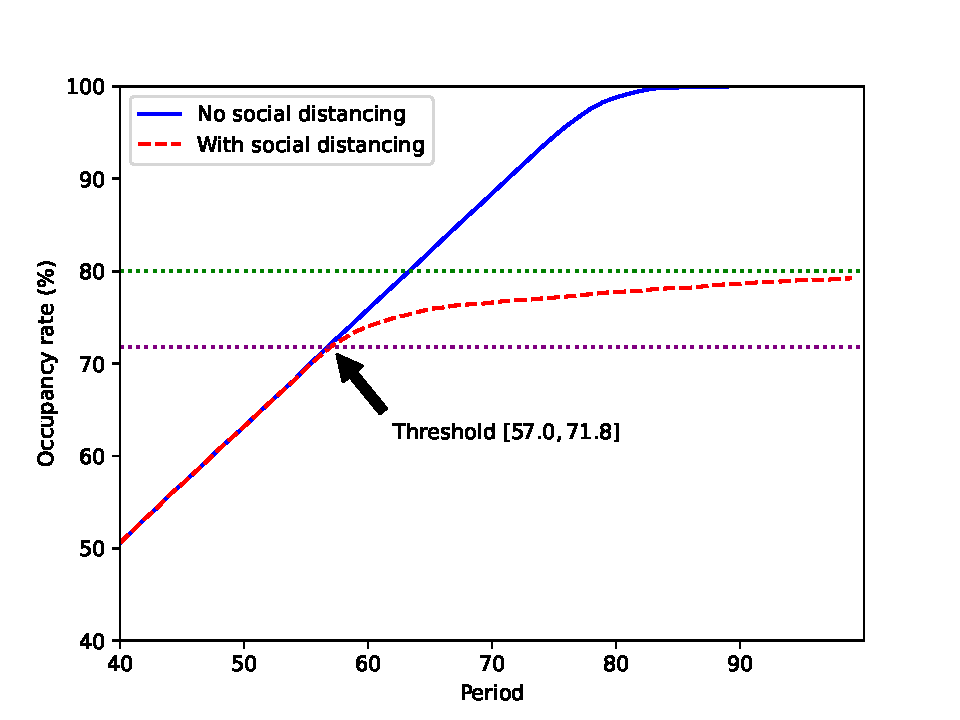
\includegraphics[scale=.40]{./Figures/occu_demand_group4.pdf}
%    \end{minipage}%
%   \begin{minipage}{.5\textwidth}
%       \centering
%   \caption{Figure 2}\label{x_demand}
% 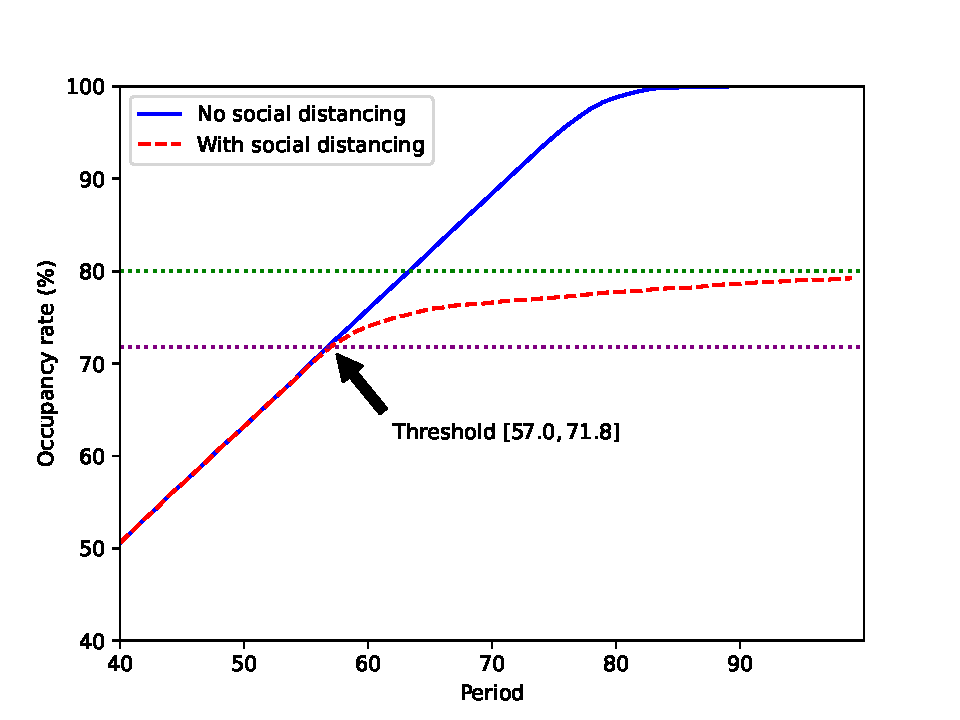
\includegraphics[scale=.40]{./Figures/occu_demand_group4.pdf} 
%   \end{minipage}
% \end{figure}

% \begin{figure}[h]
%   \centering
%   \caption{Impact of Social Distancing}    %大图名称
%   \label{occupancy_rate_demand}    %图片引用标记
%   \subfigure[]{
%     \label{x_period}
%   \begin{minipage}{7cm}
%     \centering    %子图居中
%     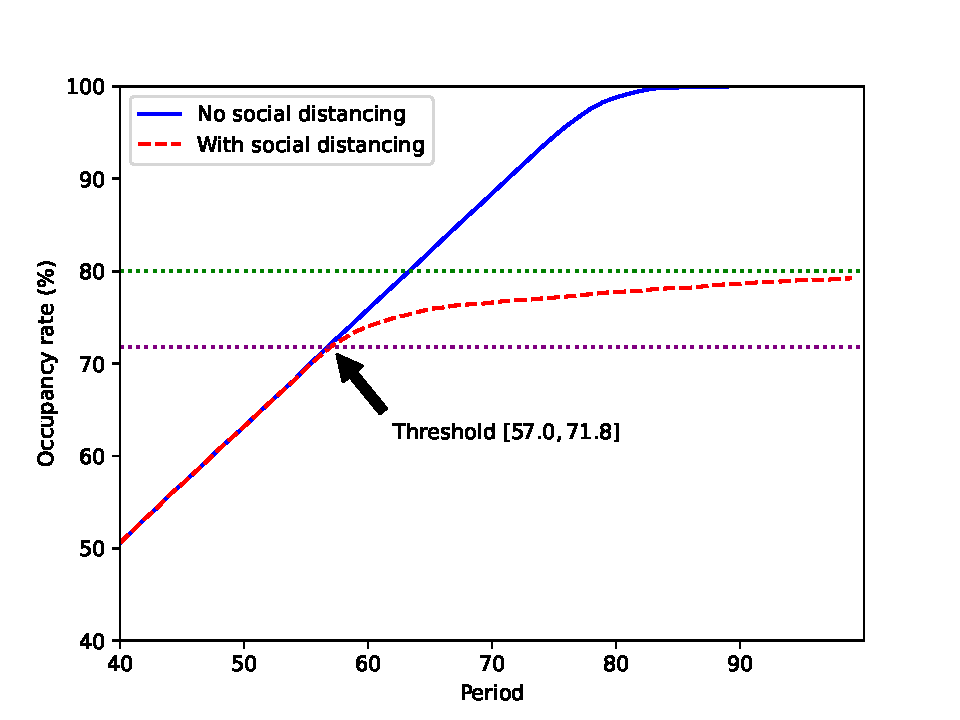
\includegraphics[scale=0.5]{./Figures/occu_demand_group4.pdf}  %以pic.jpg的0.5倍大小输出
%   \end{minipage}}
%   \subfigure[]{ %第二张子图
%   \label{x_demand}
%   \begin{minipage}{7cm}
%     \centering    %子图居中
%     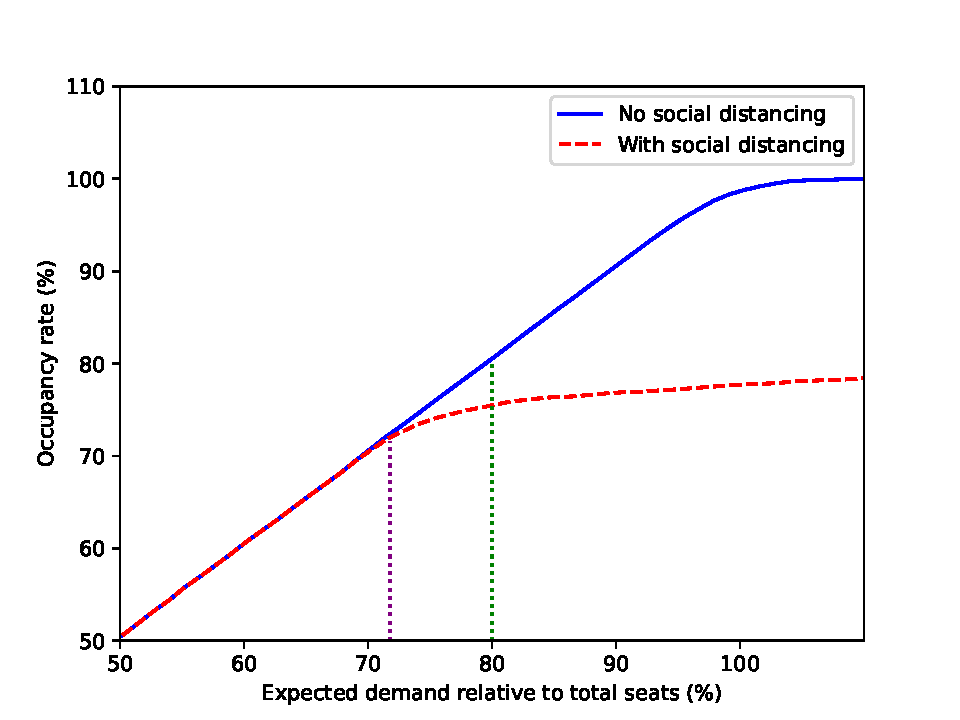
\includegraphics[scale=0.5]{./Figures/occu_gamma_group4.pdf}%以pic.jpg的0.5倍大小输出
%   \end{minipage}}
% \end{figure}

\begin{figure}[h]
  \centering
  \subfigure[]{
    \label{x_period}
    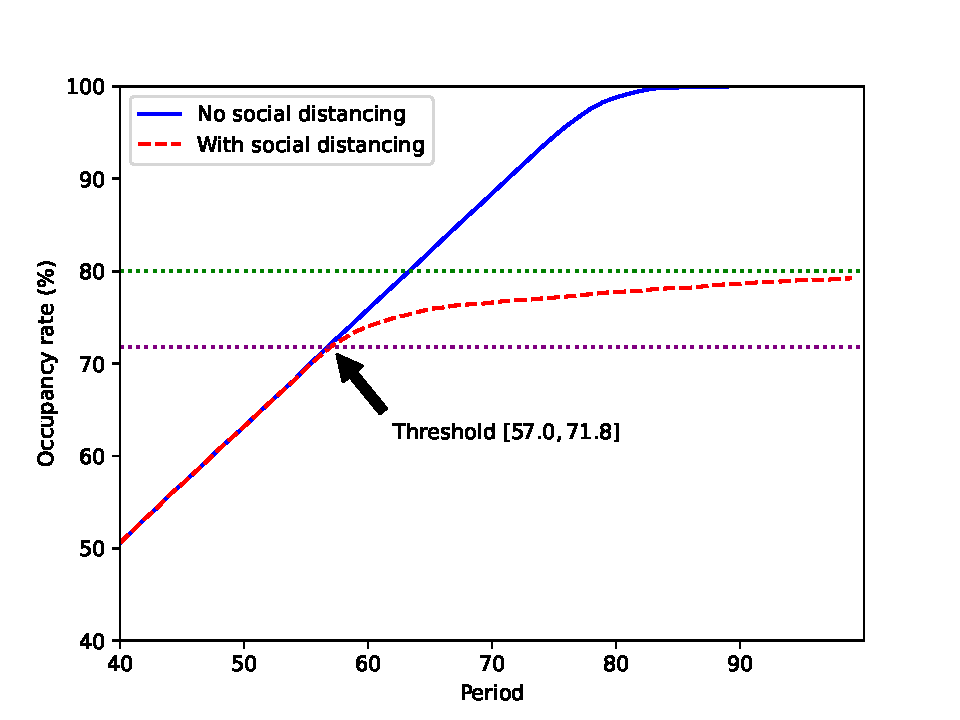
\includegraphics[width=0.45\textwidth]{./Figures/occu_demand_group4.pdf}}
    \subfigure[]{
      \label{x_demand}
      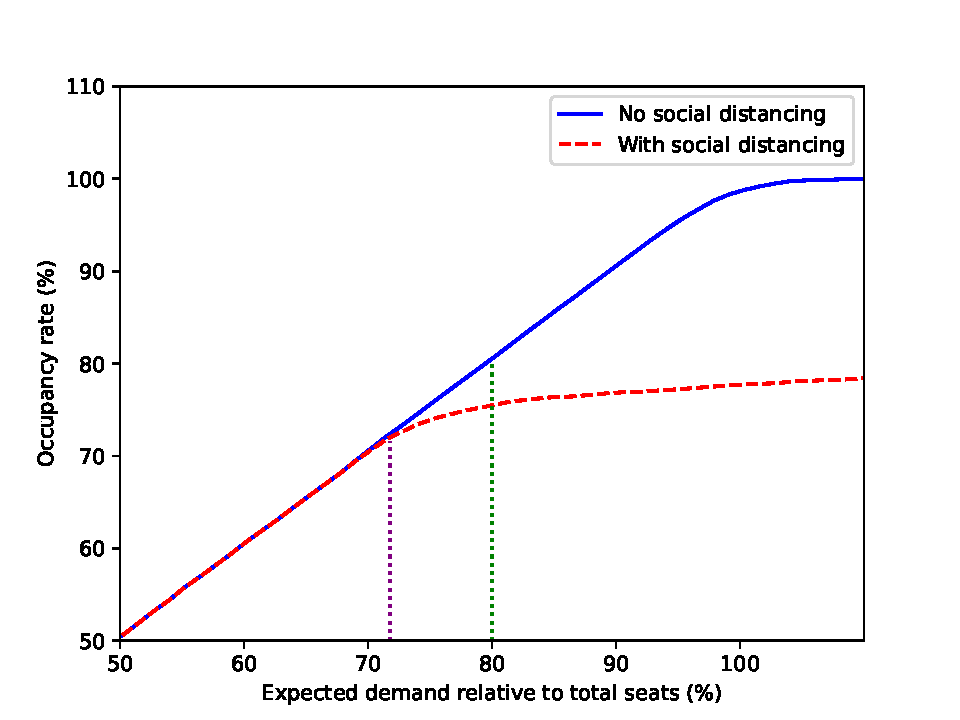
\includegraphics[width=0.45\textwidth]{./Figures/occu_gamma_group4.pdf}}
      \caption{Impact of social distancing}\label{occupancy_rate_demand}
\end{figure}

Figure \ref{x_period} illustrates the occupancy rate over period, revealing three key metrics for policy evaluation: (1) the threshold of request-volume, ${q}^{\textup{th}} = 57$, (2) the threshold of occupancy rate, $\rho^{\textup{th}} = 71.8\%$, and (3) the maximum achievable occupancy rate $\rho^{\textup{ac}} =80\%$. These metrics collectively serve as crucial indicators for assessing the effectiveness of the government policy.


% The above qualitative insights are stable concerning the tightness of the policy as well as the specific characteristics of various venues.
% Based on the above analysis, we also explore the results of different layouts, different group sizes and different social distances. 

% Since the figure about the occupancy rate over demand is similar to Figure \ref{occupancy_rate_demand}, we only use three metrics to show the results: the threshold of requests and the threshold occupancy rate, the maximum achievable occupancy rate.


Figure \ref{x_demand} presents the occupancy rate as a function of expected demand. The key distinction between Figure \ref{x_period} and Figure \ref{x_demand} lies in their respective x-axes. From a demand perspective, we observe two distinct points: for expected demand below 71.8\%, social distancing requirements impose no significant reduction in the number of assigned individuals; above this 71.8\% threshold, the performance gap between scenarios with and without social distancing becomes increasingly pronounced.

Given the conceptual similarity between period-based and demand-based occupancy rate analyses, we focus on these three metrics to concisely represent the core findings. Complete results and detailed interpretations are presented in Section \ref{perf_constraints}, which examines performance under various policy constraints.


\subsection{Robustness under Demand Distributions}
As demonstrated earlier, SPBA maintains stable performance across four distinct probability distributions. To thoroughly assess its distributional robustness, we now examine its behavior over a wide range of probability distributions. For standardized comparison, we employ two key metrics: the threshold of request-volume $q^{\textup{th}}$ and the threshold of occupancy rate $\rho^{\textup{th}}$ (noting that the maximum achievable occupancy rate $\rho^{\textup{ac}}$ is distribution-invariant).
Robustness is quantified by analyzing how these thresholds vary with the mean group size across different distributions. Finally, we provide estimates of $q^{\textup{th}}$ and $\rho^{\textup{th}}$ as functions of the mean group size.

% As previously noted, SPBA exhibits stable and consistent performance across four different probability distributions. Here, we further investigate its behavior under a large range of probability distributions. To standardize our analysis, we use the two previously defined metrics, the threshold of request-volume $q^{\textup{th}}$ and the threshold of occupancy rate $\rho^{\textup{th}}$ (note that the maximum achievable occupancy rate $\rho^{\textup{ac}}$ is distribution-independent), and evaluate robustness by observing their variations across different distributions through the mean group size. Finally, we provide an estimation of these metrics using the mean group size.

The mean group size is $\gamma = \sum_{i=1}^{M} i p_i$. We analyze the relationship between $q^{\textup{th}}$, $\rho^{\textup{th}}$ and $\gamma$ using 200 random probability distributions ($M=4$, $p_0=0$).
Figure \ref{esti_q} shows $q^{\textup{th}}$ and $\rho^{\textup{th}}$ versus $\gamma$, along with their estimates: 
$\tilde{q}^{\textup{th}} =  \frac{c_1 (1-p_0) \tilde{L}}{\gamma + \delta}$ and $\tilde{\rho}^{\textup{th}} = \frac{c_2 \gamma}{\gamma +\delta} \frac{(1-p_0) \tilde{L}}{\tilde{L}-N \delta}$, where 
$c_1$ and $c_2$ are discount factors, $\tilde{L}, \delta, N$ are defined in the problem setup, and $p_0 =0$. Using the Ordinary Least Squares regression, we obtain perfect fits ($R^{2} = 1.000$) with $c_1 = 0.9578$ and $c_2 = 0.9576$. The derivation and further details are provided in the Appendix.


\begin{figure}[H]
  \caption{The estimates of $q^{\textup{th}}$ and $\rho^{\textup{th}}$}\label{esti_q}
  \centering
    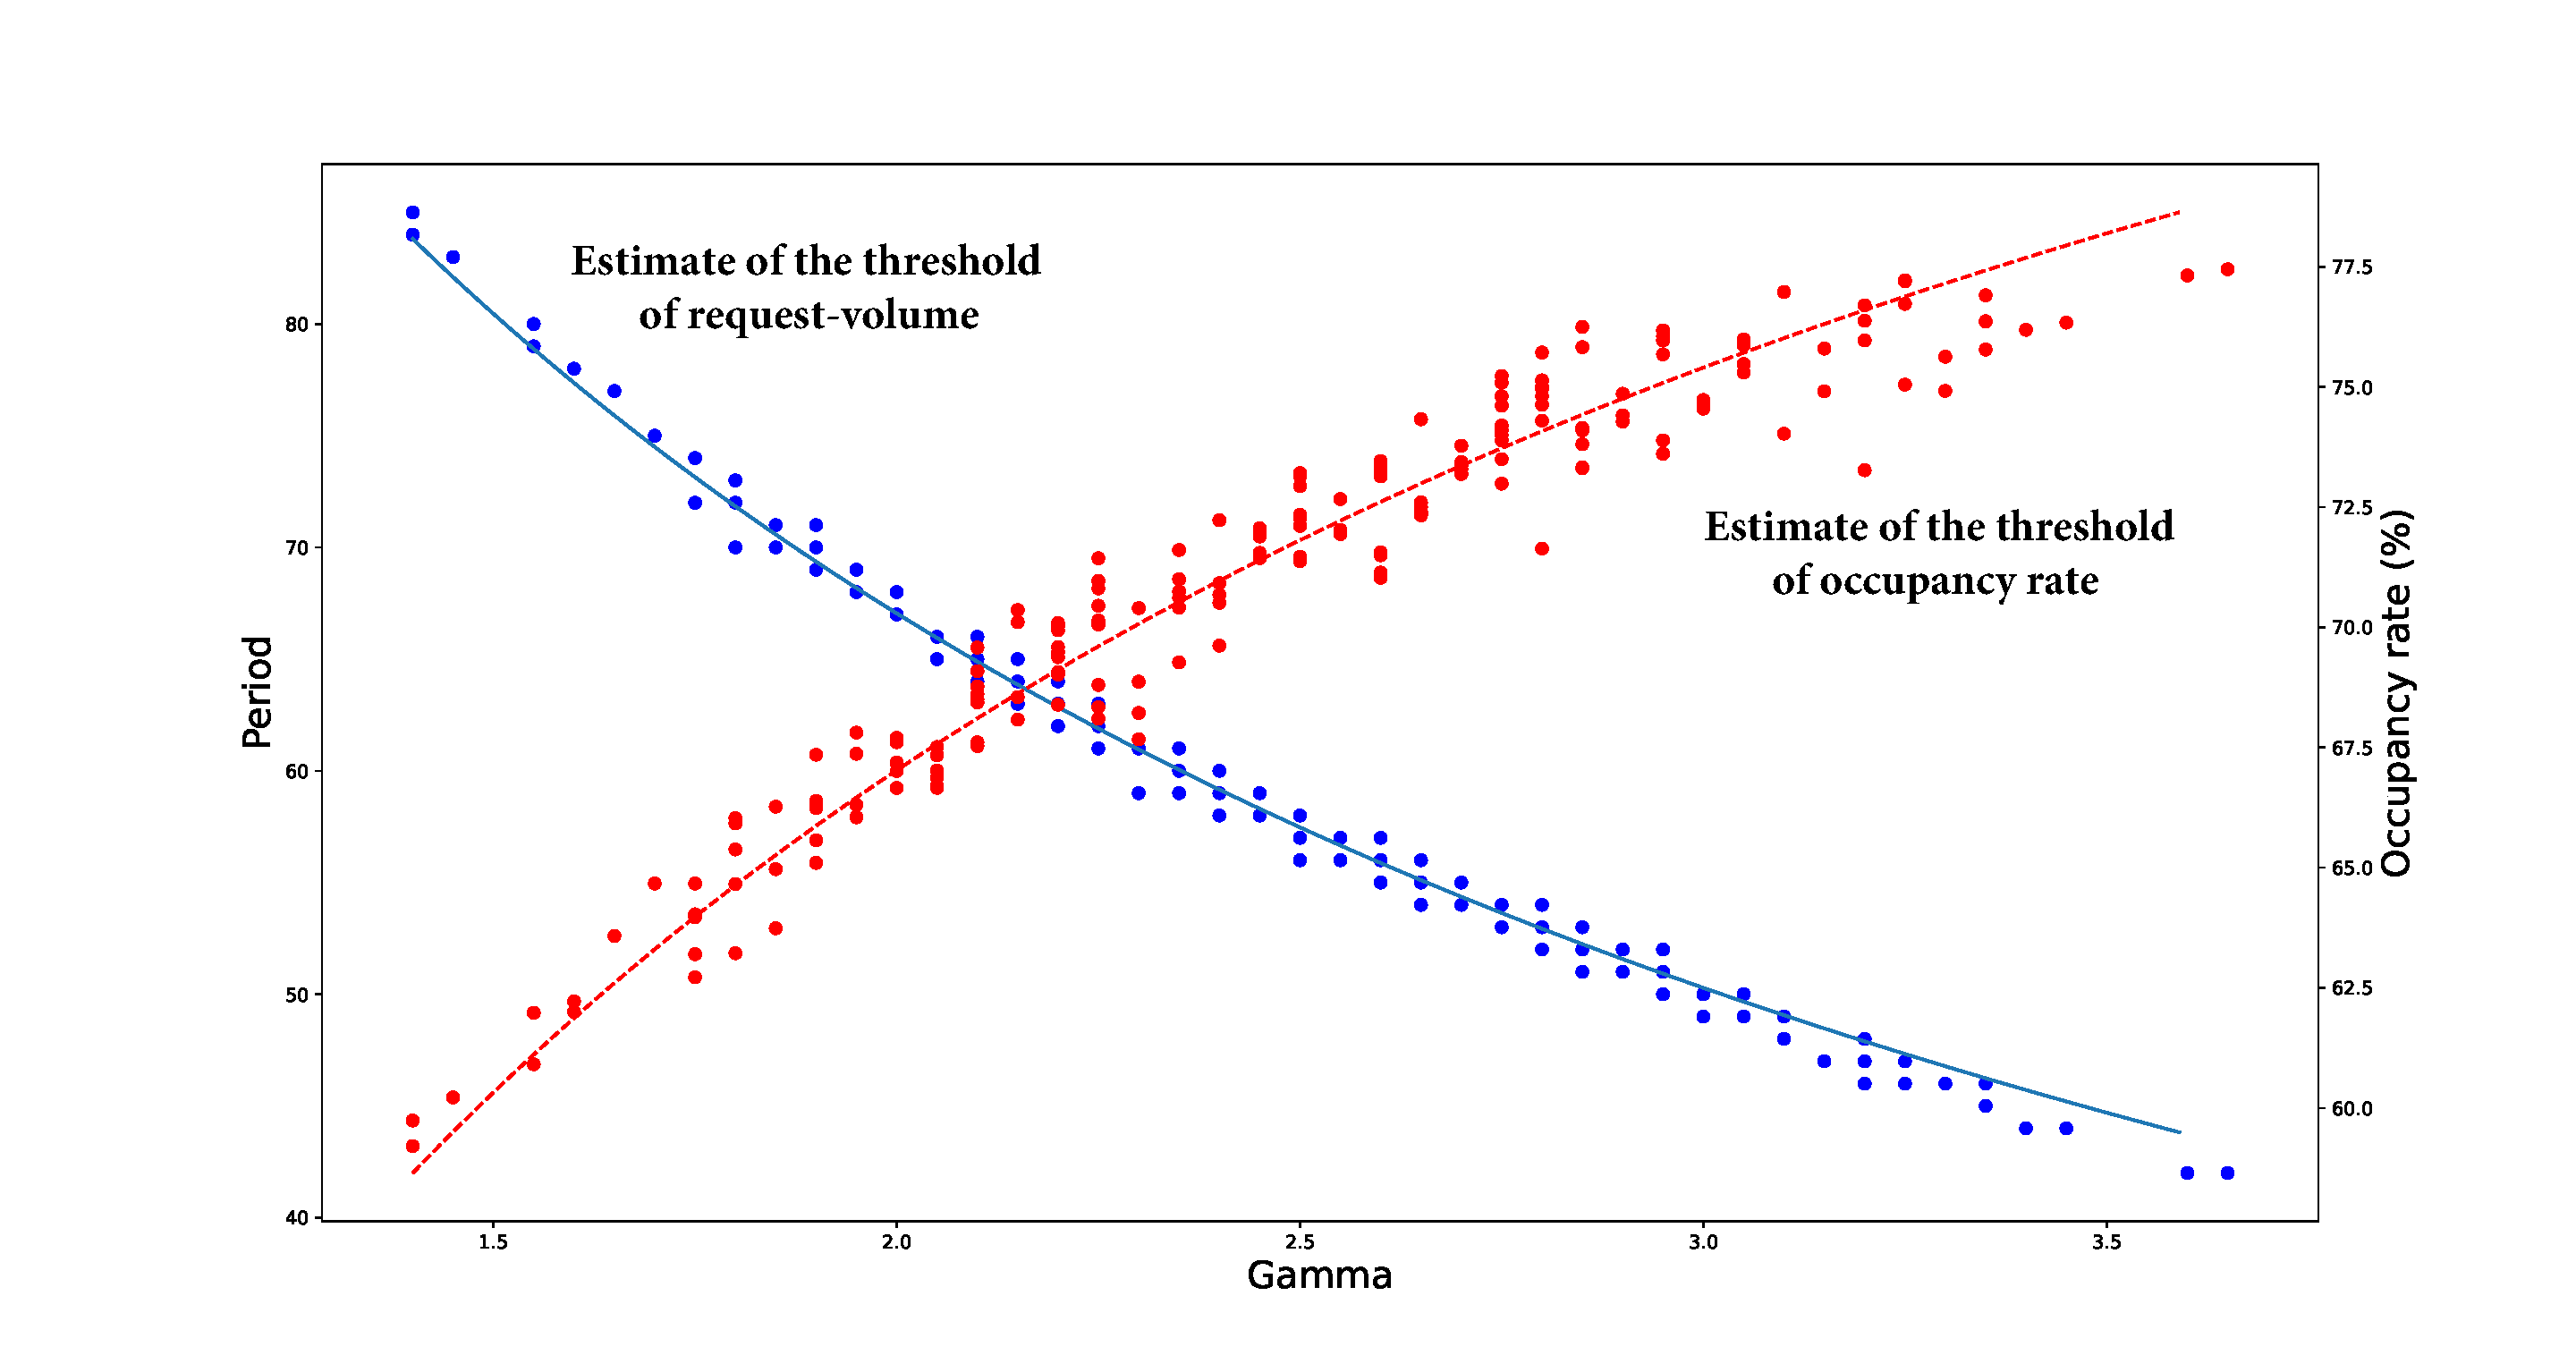
\includegraphics[width=0.95\textwidth]{./Figures/200_random.pdf}
\end{figure}

For fixed values of all other parameters, the estimated threshold of request-volume $\tilde{q}^{\textup{th}}$ decreases as the mean group size $\gamma$ increases, while the estimated threshold of occupancy rate $\tilde{\rho}^{\textup{th}}$ increases with $\gamma$. This behavior aligns with the trends observed in Figure \ref{esti_q}.


% Under the condition of fixed other parameters, the estimate of the threshold of request-volume $\tilde{q}^{\textup{th}}$ decreases with higher mean group size $\gamma$ while the estimate of threshold of occupancy rate $\tilde{\rho}^{\textup{th}}$ increases with higher mean group size $\gamma$, which follows the pattern as the figure shows.


% estimation 放在appendix  直接给结论

% We analyze how the estimates of the threshold of request-volume $\tilde{q}^{\textup{th}}$ and the threshold of occupancy rate $\tilde{q}^{\textup{th}}$ vary with respect to these parameters: mean group size $\gamma$, maximum group size $M$, physical distance $\delta$, and total size of the layout $\tilde{L}$.
% Under the condition of fixed other parameters, the estimate of the threshold of request-volume $\tilde{q}^{\textup{th}}$ decreases with higher mean group size $\gamma$ and increases linearly with the total size of the layout $\tilde{L}$. Generally, $\gamma$ increases with the maximum group size $M$ (since $\gamma = \sum_{i=1}^{M} i p_i$), leading to an indirect reduction in $\tilde{q}^{\textup{th}}$. When other parameters are held constant, the estimate of threshold of occupancy rate $\tilde{\rho}^{\textup{th}}$ increases with higher mean group size $\gamma$ (and thus with larger maximum group size $M$, if $\gamma$ raises) and decreases with larger $\tilde{L}$. The estimated $\tilde{q}^{\textup{th}}$ and $\tilde{\rho}^{\textup{th}}$ exhibit non-trivial dependencies on the physical distance parameter $\delta$ since $\tilde{L} = \sum_{j =1}^{N} L_{j}^{0} + N \delta$ couples their dynamics. 

% Assuming the discount factors $c_1$ and $c_2$ remain constant as $\delta$ increases, both $\tilde{q}^{\textup{th}}$ and $\tilde{\rho}^{\textup{th}}$ decrease monotonically, provided the total capacity satisfies $\sum_{j=1}^{N} L_{j}^{0} > N \delta$. This condition is typically met in common practical layouts.

\subsection{Performance Evaluation under Varied Constraints}\label{perf_constraints}
To comprehensively evaluate the effectiveness of government policy strictness and venue-specific characteristics, we assess the performances of four critical factors: government-mandated maximum allowable occupancy rates, variations in maximum group sizes, different physical distances ($\delta \in \{1,2\}$) and alternative seat layouts.


\subsubsection{Government-Mandated Maximum Allowable Occupancy Rates}
% add specific government perspective

Government policies may impose a maximum allowable occupancy rate ($\rho^{\textup{al}}$) to enforce stricter public health measures. The effectiveness of this policy depends on its relationship to two key metrics, threshold of occupancy rate $\rho^{\textup{th}}$ and maximum achievable occupancy rate $\rho^{\textup{ac}}$.

When $\rho^{\textup{al}} < \rho^{\textup{th}}$, only the occupancy rate requirement is binding. Once the occupancy rate reaches $\rho^{\textup{al}}$, all subsequent requests are rejected. When $\rho^{\textup{th}} \leq \rho^{\textup{al}} < \rho^{\textup{ac}}$, both maximum allowable occupancy rate and social distancing requirements jointly govern seat assignments. Again, once $\rho^{\textup{al}}$ is reached, further requests are rejected. When $\rho^{\textup{al}} \geq \rho^{\textup{ac}}$, the maximum allowable occupancy rate constraint becomes redundant because the occupancy rate will never exceed $\rho^{\textup{al}}$ under social distancing.


The conclusion can be summarized in Table \ref{tab_requirement}.
\begin{table}[ht]
  \centering
  \caption{Effectiveness of requirements}\label{tab_requirement}
  \begin{tabular}{lcc}
  \hline
  \hline
   & Social distancing requirement & Requirement of $\rho^{\textup{al}}$ \\
  %  \cmidrule(r){1-1} \cmidrule(lr){2-2} \cmidrule(lr){3-3} \cmidrule(l){4-4}
  \hline
  $\rho^{\textup{al}} < \rho^{\textup{th}}$            & Ineffective & Effective \\
  $\rho^{\textup{th}} \leq \rho^{\textup{al}} < \rho^{\textup{ac}}$  & Effective   & Effective \\
  $\rho^{\textup{al}} \geq \rho^{\textup{ac}}$                  & Effective   & Ineffective \\
   \hline
   \hline
  \end{tabular}
\end{table}


\subsubsection{Different Maximum Group Sizes and Physical Distances}
When $M$ is restricted at 3, given the probability distribution [0.12, 0.5, 0.13, 0.25], we discard the fourth component and normalize the remaining three components to generate a new probability distribution: [0.16, 0.67, 0.17]. Similarly, when $M =2$, the probability distribution is [0.19, 0.81].
We also consider the impact of different distances. We present the corresponding threshold of request-volume, the threshold of occupancy rate and the maximum achievable occupancy rate in the table below.

\begin{table}[ht]
  \centering
  \caption{Impact of $M$s and $\delta$s}
  \begin{tabular}{ccccc}
  \hline
  \hline
   $M$  & $\delta$ & $q^{\textup{th}}$ & $\rho^{\textup{th}}$ & $\rho^{\textup{ac}}$ \\
  %  \cmidrule(r){1-1} \cmidrule(lr){2-2} \cmidrule(lr){3-3} \cmidrule(l){4-4}
  \hline
   2 & 1 & 74  & 66.8 \% & 70.0 \% \\
   2 & 2 & 54  & 48.8 \% & 50.0 \% \\ 
   3 & 1 & 68  & 68.3 \% & 75.0 \% \\
   3 & 2 & 53  & 53.1 \% & 60.0 \% \\
   4 & 1 & 57  & 71.8 \% & 80.0 \% \\
   4 & 2 & 47  & 59.2 \% & 70.0 \% \\
   \hline
   \hline
  \end{tabular}
\end{table}


For the fixed physical distance $\delta$, an increase in the maximum group size $M$ generally leads to a larger mean group size $\gamma$ (since $\gamma = \sum_{i=1}^{M} i p_i$). This in turn causes the threshold of occupancy rate $\rho^{\textup{th}}$ to increase while reducing the threshold of request-volume $\tilde{q}^{\textup{th}}$, as evidenced by their respective estimates. The maximum achievable occupancy rate $\rho^{\textup{ac}}$ increases because the size of the largest pattern $\Phi(M, L_j^{0}, \delta)$ defined in Proposition \ref{lem_pattern}, is monotonically increasing in $M$.

For the fixed maximum group size $M$, the experimental results show that when the physical distance $\delta$ increases from 1 to 2 seats, both the threshold of occupancy rate $q^{\textup{th}}$ and threshold of request-volume $\rho^{\textup{th}}$ decrease, which is consistent with our estimates.
Assuming constant discount factors $c_1$ and $c_2$, both estimated thresholds $q^{\textup{th}}$ and  $\rho^{\textup{th}}$ would decrease monotonically with increasing $\delta$, provided the total capacity satisfies $\sum_{j=1}^{N} L_{j}^{0} \geq N \gamma$ (See Appendix). This condition is generally satisfied in most practical seating layouts, further validating our experimental observations. The maximum achievable occupancy rate, $\rho^{\textup{ac}}$, decreases since $\Phi(M, L_j^{0}, \delta)$ is monotonically decreasing in $\delta$.
 
% as the physical distance $\delta$ increases from 1 to 2 seats, both the threshold of occupancy rate $q^{\textup{th}}$ and threshold of request-volume $\rho^{\textup{th}}$ decrease (consistent with the analysis in the estimation). 

% Assuming the discount factors $c_1$ and $c_2$ remain constant as $\delta$ increases, both $\tilde{q}^{\textup{th}}$ and $\tilde{\rho}^{\textup{th}}$ decrease monotonically, provided the total capacity satisfies $\sum_{j=1}^{N} L_{j}^{0} > N \delta$. This condition is typically met in common practical layouts.



% We observe that larger group sizes correspond to higher largest occupancy rates under the same seat layout. However, the gap point and occupancy rate for larger group sizes do not necessarily increase correspondingly. The explanation for this is that as larger groups are allowed to be accepted, seat allocation makes it difficult to achieve a full pattern for each row. Thus, there will be a decrease in both gap points and occupancy rates, i.e., the impact of social distancing will manifest at an earlier period.

% The insight is although allowing larger groups will increase the largest occupancy rate, the impact of social distancing will become evident at an earlier period. Specifically, if demand is low or if the managers wish to avoid rejecting a significant number of customers, they can set a smaller group size limit. Conversely, when demand is high, a larger group size limit can be set to accommodate more customers.

% \subsubsection{Different Physical Distances}
% The following figure illustrates the occupancy rate with different physical distances over the period.

% \begin{figure}[h]
%   \caption{Impact of different distances}\label{result_dis}
%   \centering
%     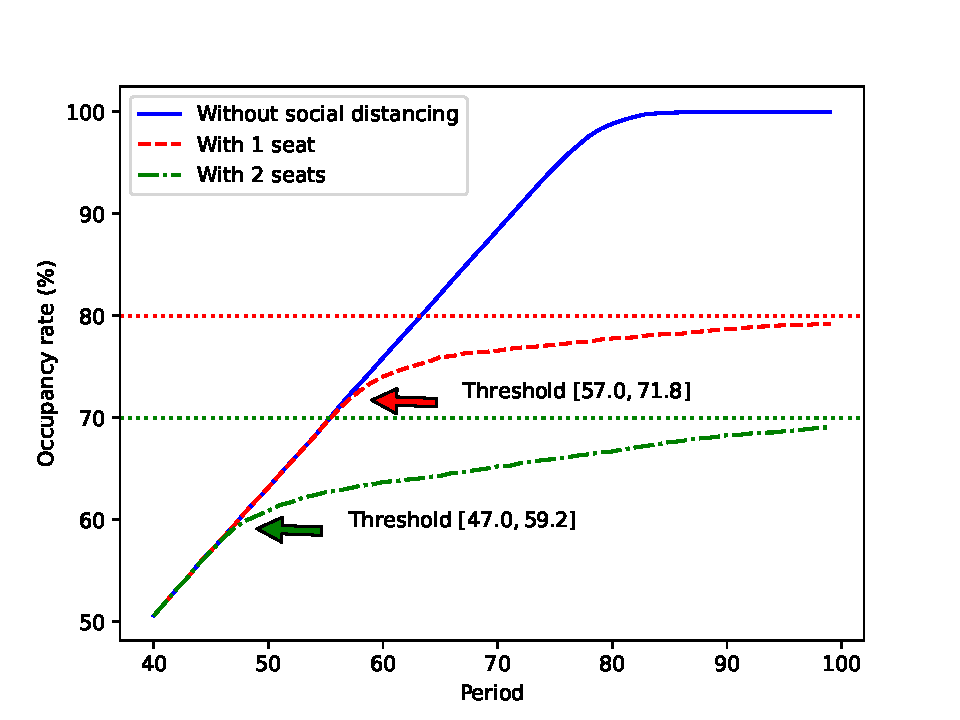
\includegraphics[width=0.7\textwidth]{./Figures/distance_3.pdf}
% \end{figure}

% The threshold of request-volume, the threshold occupancy rate and the maximum achievable occupancy rate are shown in the table below.

% \begin{table}[ht]
%   \centering
%   \caption{Gap points and occupancy rates of $\delta$s}
%   \begin{tabular}{c|ccc}
%   \hline
%    $\delta$  & Gap point & Threshold occupancy rate & Maximum achievable occupancy rate \\
%   %  \cmidrule(r){1-1} \cmidrule(lr){2-2} \cmidrule(lr){3-3} \cmidrule(l){4-4}
%   \hline
%    1 &  57  & 71.76 \% & 80 \% \\
%    2 &  47  & 59.16 \% & 70 \% \\
%    \hline
%   \end{tabular}
% \end{table}

\subsubsection{Alternative Seat Layouts}
We experiment with several realistic seat layouts selected from a theater seat plan website, choosing five layouts labeled A, B, C, D, and E. Layouts A, D, and E are approximately rectangular, Layout C is a standard rectangular layout, and Layout B is irregular. In these layouts, wheelchair seats and management seats are excluded, while seats with sufficient space for an aisle are treated as new rows. The specific layouts are detailed in Appendix.

The occupancy rate over demand follows the typical pattern of Figure \ref{occupancy_rate_demand}. The threshold of request-volume, the threshold of occupancy rate and the maximum achievable occupancy rate are also given in the following table. The maximum achievable occupancy rate can be calculated from Proposition \ref{lem_pattern}.

\begin{table}[ht]
  \centering
  \caption{Impact of the layouts}
  \begin{tabular}{cccc}
  \hline
  \hline
   Layout & $q^{\textup{th}}$ & $\rho^{\textup{th}}$ & $\rho^{\textup{ac}}$ \\
  %  \cmidrule(r){1-1} \cmidrule(lr){2-2} \cmidrule(lr){3-3} \cmidrule(l){4-4}
  \hline
   A & 36 & 72.3 \% & 82.4 \% \\
   B & 38 & 75.8 \% & 84.1 \% \\
   C & 32 & 72.8 \% & 80.0 \% \\
   D & 43 & 74.1 \%  & 83.6 \% \\
   E & 102 & 72.4 \% & 81.7 \% \\
   \hline
   \hline
  \end{tabular}
\end{table}

While the venue layouts may differ in shapes (rectangular or otherwise) and row configurations (varying lengths), the maximum achievable occupancy rate $\rho^{\textup{ac}}$ do not shows the deterministic variation pattern.

Consistent with our estimates, the threshold of request-volume $q^{\textup{th}}$ follows $\tilde{q}^{\textup{th}} =  \frac{c_1 (1-p_0) \tilde{L}}{\gamma + \delta}$, exhibiting a positive correlation with total size of the layout $\tilde{L}$. 

While the estimate shows that $\tilde{\rho}^{\textup{th}} = \frac{c_2 \gamma}{\gamma +\delta} \frac{(1-p_0) \tilde{L}}{\tilde{L}-N \delta}$ should decrease with increasing $\tilde{L}$, in practice this variation becomes negligible as the ratio $\frac{\tilde{L}}{\tilde{L}-N\delta}$ remains nearly constant for typical venue sizes. This explains the observed lack of deterministic variation in 
$\rho^{\textup{th}}$ across layouts with different seating configurations.


% $\tilde{\rho}^{\textup{th}} = \frac{c_2 \gamma}{\gamma +\delta} \frac{(1-p_0) \tilde{L}}{(1-p_0) \tilde{L}-N \delta}$, the threshold of occupancy rate $\rho^{\textup{th}}$ decreases with increasing $\tilde{L}$, though this variation becomes negligible when the ratio $\frac{\tilde{L}}{\tilde{L}-N\delta}$ changes little. Consequently, for practical layouts with differing total seats and row arrangements, the threshold of occupancy rate $\rho^{\textup{th}}$ shows no deterministic variation pattern.

% the threshold of occupancy rate $\rho^{\textup{th}}$ 

